\documentclass[letterpaper, 10 pt, journal, twoside]{IEEEtran}
%\documentclass[journal]{IEEEtran}
\usepackage[maxnames=6,firstinits=true,doi=false,url=true,isbn=false]{biblatex}
\addbibresource{IROS.bib}
\usepackage{array}
\usepackage{graphicx}
\usepackage{amsmath}
\usepackage{amssymb}
\usepackage{color}
\usepackage{threeparttable}
\usepackage{balance} %balance columns
\usepackage{todonotes}
\hyphenation{op-tical net-works semi-conduc-tor}

%\pagenumbering{gobble} %suppresses page numbers

\begin{document}
\title{A Multi-Agent Systems Approach to Test Generation for Simulation-based Autonomous Vehicle Verification}
\author{Greg~Chance$^{1}$, 
Abanoub~Ghobrial$^{1}$, 
Severin Lemaignan$^{2}$,
Tony Pipe$^{2}$,
Kerstin Eder$^{1}$%~\IEEEmembership{Senior Member,~IEEE}, 


%\thanks{Manuscript received: Feb 23, 2018; Revised: May 21, 2018; Accepted: Jun 21, 2018.}
\thanks{$^{1}$Abanoub Ghobrial, Greg Chance and Kerstin Eder are with the University of Bristol, Bristol, UK {\tt\footnotesize \{greg.chance, abanoub.ghobrial, kerstin.eder\}@bristol.ac.uk}}%
\thanks{$^{2}$Severin Lemaignan and Tony Pipe are with the Bristol Robotics Laboratory, University of the West of England, Bristol, UK {\tt\footnotesize \{severin.lemaignan, tony.pipe\}@brl.ac.uk}}%
}
% The paper headers
%\markboth{Submission to IEEE AI Testing 2019}%
%{Shell \MakeLowercase{\textit{et al.}}: Bare Demo of IEEEtran.cls for IEEE Journals}
%\markboth{IEEE Robotics and Automation Letters. Preprint Version. Accepted June, 2018}
%{Chance \MakeLowercase{\textit{et al.}}: ``Elbows Out" - Predictive Tracking of Partially Occluded Pose} 
\maketitle

\begin{abstract}
Simulation-based verification is beneficial for assessing otherwise dangerous or costly on-road testing of autonomous vehicles (AV). This paper addresses the challenge of efficiently generating effective tests for simulation-based AV verification using software testing agents. The multi-agent system (MAS) programming paradigm offers rational agency, causality and strategic planning between multiple agents. We exploit these aspects for test generation, focusing in particular on the generation of tests that trigger preconditions of assertions. On the example of a key assertion we show that, by encoding a variety of different behaviours respondent to the agent's perceptions of the test environment, the agent-based approach generates twice as many effective tests than pseudo-random test generation, while being  both scalable and efficient. Moreover, agents can be encoded to behave naturally without compromising the effectiveness of test generation. Our results suggest that generating tests using testing agents significantly improves upon random and simultaneously provides more realistic driving scenarios.
%
%Our results suggest that generating tests using testing agents allows engineers to reach edge cases and rare events more easily. %
% GC:

% Simulation based verification for autonomous vehicles (AV) is beneficial for assessing otherwise dangerous or costly on-road testing. The multi-agent system (MAS) programming paradigm was used in the context of AV verification to explore the potential for test generation. Generating tests using autonomous agents has many benefits including scalability and engineering efficiency. We explore different agent behaviours towards the goal of assertion coverage through a simple example. By provoking behaviours based on the agents perceptions of the scenario we show that the agent-based test generation out-performs random agent actions by over 50\% in terms of test generation accuracy. MAS test generation shows promising results for simulation based verification allowing engineers to exploit edge cases and rare events more easily. 

\end{abstract}
\begin{IEEEkeywords}
Test Generation, Simulation, Autonomous Driving, Verification, Multi-Agent System, Testing Agent
\end{IEEEkeywords}
\IEEEpeerreviewmaketitle

%------------------- Intro -----------------------------
\section{Introduction}
%\IEEEPARstart{A}{n} agent is a computational mechanism that exhibits a high degree of autonomy, performing actions in its environment based on information received \cite{Panait2005}. A multi-agent system contains one or more agents whom interact but may not share information about the environment that is known by a single agent. This individual level information bias may lead to emergent properties in the multi-agent group behaviour as a result of the interaction between agents.

%----------------------------------------------------------
% What is verification
\IEEEPARstart{V}{erification} is the process used to gain confidence in the correctness of a system with respect to its requirements~\cite{bergeron2012writing}. Testing is a technique that can be used to achieve this by showing that the intended and actual behaviours of a system do not differ and detecting failures against the requirements in the process~\cite{utting2012taxonomy}.



%----------------------------------------------------------
% What is the role of testing
% above
% Actual quote is: "Verification is a process used to demonstrate that the intent of a design is preserved in its implementation", [Bergeron].

%----------------------------------------------------------
% The principle of verification based testing
Using simulation to test autonomous driving functions in safety critical scenarios benefits from full control over the environment, where road layouts, weather conditions, a variety of road users and other %traffic participants
driving scenario parameters 
can be directed to achieve specific test targets. %
%
% These tests may look to convince auditors of the functional safety of the vehicle or whether it complies with commonly agreed upon road conduct, such as the Vienna convention~\cite{ViennaConv}, interpreted locally by each country, e.g.\ the UK Highway Code~\cite{codes2011highway}. In addition, there are also road traffic laws and penalties, e.g.~\cite{RoadTraffic1988}, and unwritten rules or social conventions~\cite{}. 
%
These tests may aim to provide evidence to regulators of the functional safety of the vehicle or its compliance with commonly agreed upon road conduct, such as the Vienna convention~\cite{ViennaConv}, typically implemented at national level as a set of rules~\cite{codes2015highway}, road traffic laws and penalties~\cite{RoadTraffic1988}.
%
%These may be culturally or geographically different, e.g.\ flashing headlights to override junction priorities to give way to another driver.


%----------------------------------------------------------
% The Test Generation challenge and its automation
Verification of complex systems is challenging. In semiconductor design, for
example, it has long been recognised that verification can take up to 70\% of
the design effort~\cite{arden2002international}, with the largest part still
being achieved with simulation-based techniques. 
%
The testbench is the code used to drive a stimulus sequence into the Design
under Verification (DUV) while observing input protocols. It also records
coverage and checks the DUV's response. The testbench provides a completely
closed environment from the DUV's perspective. Simulators are used to execute
testbenches. Automation plays a critical role in achieving verification targets
efficiently and effectively.

Coverage-driven verification is a systematic, goal-directed simulation-based
verification method~\cite{HVC2015} that offers a high degree of automation and
is capable of exploring systems of realistic detail under a broad range of
environment conditions.
%
Because exhaustive simulation is intractabe due to the vast parameter space,
the remaining challenge is in strategically selecting the (ideally smallest set
of) test cases that result in the highest level of confidence in the design's
correctness.
%
Automating test generation has been the focus of research for decades, giving
rise to a variety of coverage-directed stimulus generation techniques that
exploit formal methods, genetic programming and machine learning~\cite{Ioannides:2012}. 

Compared to semiconductor design verification, AV verification faces even bigger challenges, including automatic test generation. 
%
It is well known that few of the valid tests are actually interesting from a verification point of view. 
Estimates vary, but demonstrating AV safety with a confidence of 95\% that the failure rate is at most 1.09 fatalities per 100 million miles driven would take 275 million miles, equivalent to 12.5 years for a fleet of 100 AVs~\cite{kalra2016driving}. %
%
This figure is based on the number of roads fatalities in the US, and would
need to be adjusted taking into consideration local statistics on road safety,
e.g.\ the number of road fatalities per billion vehicle-km in the UK has been
half that of the US in 2018~\cite{ITFroadSafety2018}.
%
Ways must be found to test the scenarios of interest without needing millions of miles of driving or billions of miles of simulated driving~\cite{korosec2019waymo}.
%
In particular, simulation-based testing offers the opportunity to increase the number of otherwise rare events~\cite{Koopman2018} in order to determine whether the AV handles such rare events appropriately. 
%
% For the public to gain trust in autonomous vehicles (AV), the manufacturers must demonstrate that their AVs comply with, amongst many things, road safety requirements. 
% While on-road testing will contribute significantly towards AV verification, testing in simulation has complimentary benefits as it offers a safe and effective environment. 
%
% Testing in simulation enables many processes to be automated which may be convenient for ensuring compliance during version change, e.g. software updates or patches to the vehicle.
% But automation can also apply to not just the process but the method of test generation which is the focus of this paper.


\begin{figure}[!t]
	\centering
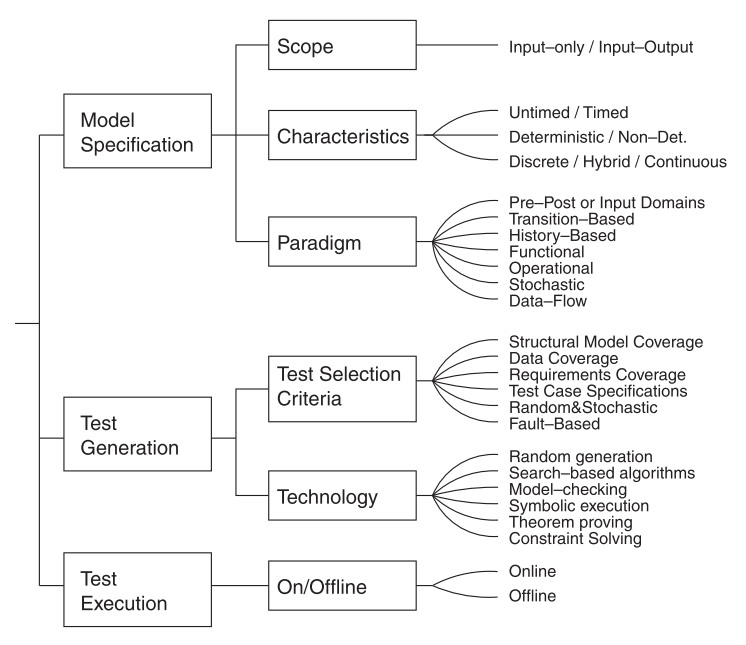
\includegraphics[width=0.48\textwidth]{taxonomy.png}
	\caption{Taxonomy of model-based test generation, from~\cite{utting2012taxonomy}}
	\label{taxonomy}
\end{figure}


%----------------------------------------------------------
% The AV as a DUT/SUV/DUV
Considering the AV as a DUV, the challenge is to generate tests that interact with the AV over a period of time, thereby creating an environment in which the AV needs to respond to the received stimulus while making progress towards its destination. 
%
As such, the AV can be classed as a \textit{responder\/} DUV, i.e.\ a DUV that reacts to lower-level stimulus observed on its interfaces with the surrounding environment in order to maintain legally correct driving behaviour and follow the social norms associated with road traffic.
%
% RESPONDER (https://verificationacademy.com/cookbook/doc/glossary/responder): A verification component which, similar to a driver, interacts with a lower level of abstraction such as the individual signals on a protocol interface, in order to participate in a protocol. Unlike a driver, responders do not initiate stimulus traffic from a sequence, they respond (slave-like) to traffic observed on the interface in order to maintain legal protocol. Their execution may be controlled by configuration (specifying how they are to respond in general) including some constrained randomization possible within the allowed configuration space, or by sequences of configuration changes (altering the way they respond in a controlled way), or by maintaining some state, e.g. a memory model or register model, which reflects persistent data values deposited by earlier traffic and subsequently retrieved accurately by the responder.
%
%----------------------------------------------------------
% The promise of AGENCY to address verifying responders
This paper investigates the benefits of introducing \textit{agency} into the verification environment in order to address the challenges of verifying the responder DUV. 
%
Each software agent is tasked with specific goals that aim to achieve verification objectives, e.g.\ reaching coverage targets.
%
A set of software agents can then be directed to interact, coordinating their behaviour in response to the AV's observed actions in order to increase the likelihood of rare events occurring during simulation to reach coverage targets faster.
%
%----------------------------------------------------------
% Research Questions
% -new test generation technique
Our key research question is: what are the benefits of using agent-based test generation for the verification of AVs in simulation?
%
In particular, we are interested in how agent-based test generation compares to pseudo-random test generation techniques wrt.\ the following criteria for a 'good' test case, which are inspired by~\cite{fewster1999software}:
%
%----------------------------------------------------------
% What makes a good test case?
% The challenge here is to find the correct stimulus for the AV which is described by the test case. 
%
\textit{effectiveness} in detecting defects, \textit{efficiency} in minimising the number if tests required to achieve verification goals, \textit{economy} in terms of resource usage during verification as well as during the analysis of the verification results, and also \textit{robustness} towards changes. 
%
Our results suggest that generating tests using testing agents significantly improves upon random and simultaneously provides  driving scenarios that are more realistic than those obtained by random test generation.

We regard agent-based test generation as a contribution to the well-established model-based test generation paradigm. A taxonomy of model-based test generation from~\cite{utting2012taxonomy} is given in Figure~\ref{taxonomy}.
%
The agent-based technique creates two new entries in that taxonomy, a new Paradigm under Model Specification, \textit{Agent-based}, and a new Technology under Test Generation, \textit{Planning}.
%
In this paper we use an agent-based model to specify the test environment of the AV. Agency is given to the key dynamic entities in the test environment that interact with the AV, in our case pedestrians. Planning is then employed to generate tests based on the multi-agent system that represents the test environment. Note that other test generation techniques, such as random generation, which we use as baseline for evaluation, or model checking~\cite{Bordini2006}, can also be applied to an agent-based model.	

This paper is structured as follows. In the next section we introduce the testbench architecture used in our experiment and the terminology we will adopt throughout the paper. In Section~\ref{s:background} we review related work on test generation for simulation-based AV verification. Section~\ref{s:case-study} presents our case study, which is centred around test generation for a collision avoidance scenario. Results are presented and discussed in Section~\ref{s:results}. We conclude in Section~\ref{s:conclusion} and give an outlook on future work. 

\section{Testbench Architecture and Terminology}\label{s:testbench}
%----------------------------------------------------------
% Test Bench Architecture
The proposed test bench, see Fig.~\ref{testbench}, is driven by a specification for the experiment which defines the scene and scenario including all dynamic actors. 
%
The experiment or test case specification specifies the test inputs, execution conditions for an item to be tested~\cite{StandardsBoard1990} to the test bench. 
%
The Vehicle Behaviour Interface (VBI) connects the AV controller to the simulator. It provides the simulator with the driving decisions of the AV and forwards updates on the scene to the AV controller. 
%
A geospacial database logs the AV and all other actors to enable post-simulation assertion checking. % as described in~\cite[ref our test bench paper]. 

%----------------------------------------------------------
% Scene, Scenario definitions
As well defined in~\cite{Ulbrich2015}; Scene refers to all static objects including the road network, street furniture and a snapshot of any dynamic elements. Any dynamic element whose actions or behaviour may change with respect to time are considered actors which may include other road vehicles, pedestrians and traffic signals. 
%
A situation is defined as the subjective conditions and determinants for behaviour at a particular point in time. 
%
The scenario is defined as a temporal development between several scenes which may be specified by specific goals and values.

\begin{figure}[!t]
	\centering
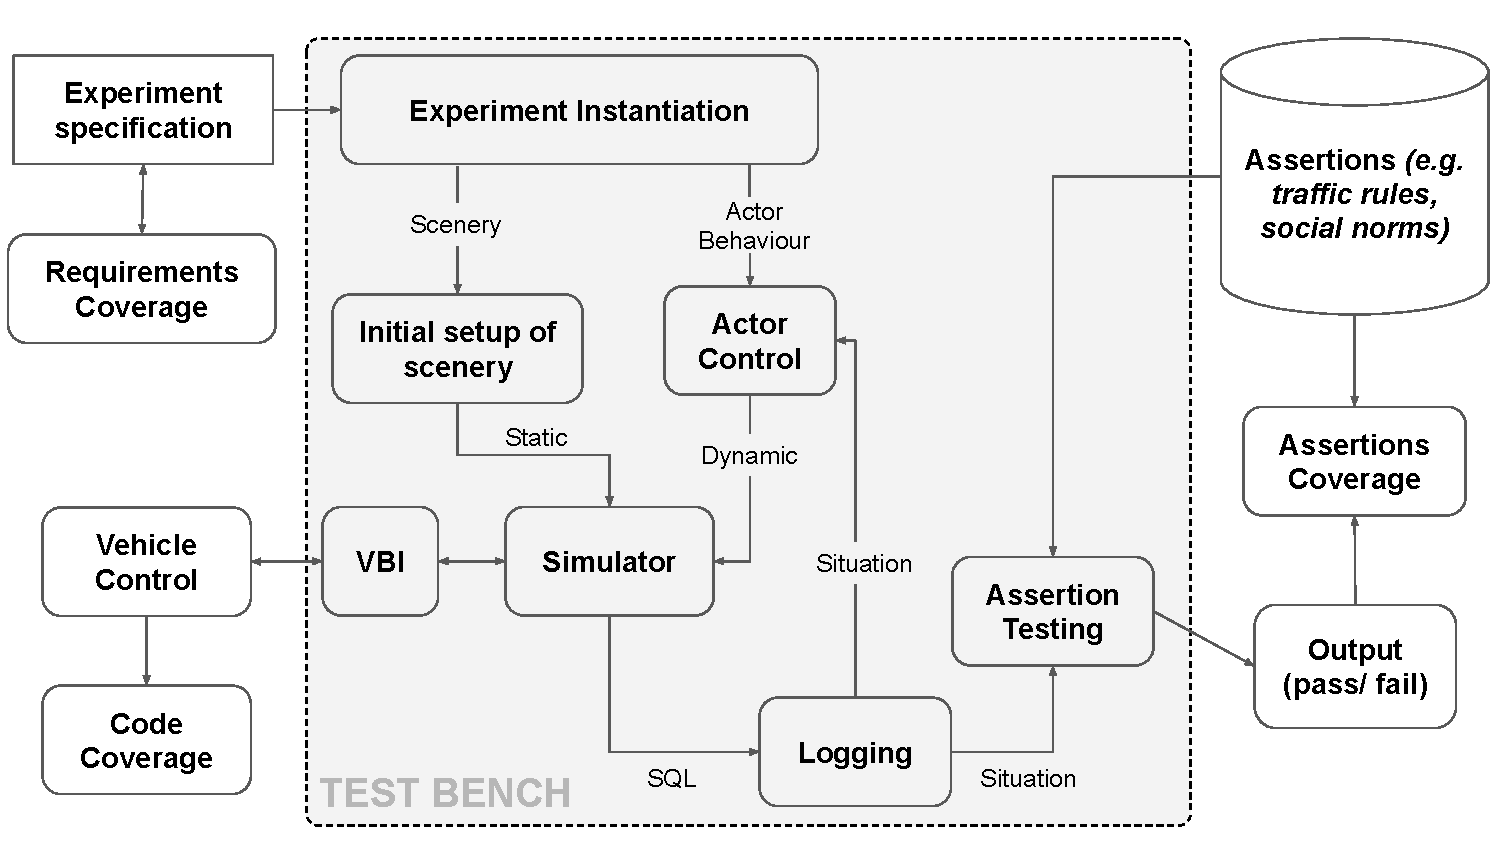
\includegraphics[width=0.48\textwidth]{TestBenchMonotone.pdf}
	\caption{Test bench design.}
	\label{testbench}
\end{figure}

%
The test case specification may be generated in a number of ways familiar to the verification engineer. Tests may be manually generated which will be both valid and accurate in producing the desired test conditions but at the highest cost. Random methods are usually employed at an early stage of testing to get coverage quickly but potentially suffer from generating invalid tests or tests that are not interesting, where interesting in this case refers to exercising the decision making processes of the AV. Model-based test generation sits between these methods in terms of validity of tests and the cost to produce them. Model-based testing requires a model that encodes the behaviour of the test environment then used to generate tests for execution.
%
%----------------------------------------------------------
% Summary
The proposed method focuses on the development between scenes dictated by the goals or values of the dynamic actors in the scene. A suitable framework for this approach to control is the Multi-Agent Systems paradigm. 



%----------------------------------------------------------
% MAS background and use of MAS for TG (morse, norway - in email from KE)
\section{Multi-Agent Systems}

Georgeff and Lansky were key in the development of the belief-desire intention (BDI) agent programming approach~\cite{georgeff1987reactive} and also in the early work of multi-agent systems~\cite{georgeff1988communication}.
%
%Waters et al. describe improvements to BDI agents through modifying the intention selection method using priority-based schedulers. They propose \textit{enablement checking} where an agent should not attempt to pursue an intention if there is no way to accomplish it and claim substantial benefits can be gained when 'running vulnerable programs in dynamic environments'~\cite{Waters2015}. This is an interesting approach and highly relevant to the AV verification domain potentially preventing unwanted emergent agent behaviour such as 'zombie attack'.
%
%Schut et al. argue that the intentions of a rational agent are not static and should reconsider their intentions if they cannot be acted upon~\cite{Schut2004}. Considering the degree of inaccessibility of the goal and cleverly considering intention reconsideration as an action the authors use POMDP to find the optimal intention reconsideration policy. Faccin et al. propose higher level intention selection using a meta-model to learn and predict plan outcomes~\cite{faccin2015bdi} demonstrating positive experimental results.
%
%----------------------------------------------------------
% Automated TG
Automatically generating stimulus that will increase functional coverage is a key challenge in simulation based verification and is a key vitue of constrained pseudo-random techniques. But such techniques are also far from completely automated, as the verification engineer must supply the suitbale constriants which become ever more complex in real driving scenarios. Feedback based coverage-driven generation (CDG) employs machine learning techniques to automatically generate tests based on rewards from a neural network or Markov Decision Process (MDP). Inductive Logic Programming based Coverage Driven Generation (ILP-CDG) has been shown to improve coverage closure by training on data generated during psuedo-random test generation and learning rules to constrain subsequent simulations~\cite{Eder2007}.
%
%----------------------------------------------------------
% MAS Automated TG
Combining the BDI framework with an automated test generation approach leads to the idea of a software agent capable of generating tests. Intelligent agents have been used in the human robot interaction (HRI) domain with a coverage feedback driven generation approach using reinforcement learning to explore collaborative manufacturing~\cite{Araiza-Illan2016}. The idea of a test agent has also been proposed by Enoiu et al.,~\cite{Enoiu2019} for regression testing although more for test selection from a library rather than generation, where agents decide what tests to execute and with what prioritisation and includes inter-agent messaging.
%
%----------------------------------------------------------
% MAS Automated TG
Hawkins et al.~\cite{hawkins2019situation} use the Multi-Agent Simulator Of Neighbourhoods (MASON) platform to filter situation coverage from a small model for an autonomous robot (AR) to efficiently ensure parameter combinations are not repeated.

%----------------------------------------------------------
% lead from MAS background into literature



%------------------- Related -----------------------------
\section{Related Work}\label{s:background}
% Describe conventional methods for test generation for verification, e.g. formal methods, random methods, hand-written tests.
% Discuss the ways that you can generate tests 1)use random 2) use engineers to write tests 3)AI/ML methods ...

A good overview of the challenges currently faced in software testing of autonomous vehicles are well document by Koopman highlighting the importance of fault injection into the testing domain~\cite{Koopman2016} and how to decide what aspects of the system need to be tested in the areas of operational design domains, event detection and vehicle manoeuvres~\cite{Koopman2019}. 
%
Describing a driving scene in natural language has been shown to be an effective framework for scenario generation which can also be automated based formalised rules and knowledge~\cite{Bagschik2018} or even evolving from ISO safety standards~\cite{Menzel2018}. 
%
Hallenbach et al. take the approach to test generation of developing composite metrics for traffic quality and using them to determine if a scenarios is `critical' or not and therefore worth exploring further~\cite{Hallerbach2018}. 
%
Generating targeted test cases can be a more efficient way to get complete coverage. By finding tests that exercise the complete decision making domain we can do away with the `unnecessary miles' of testing precisely explored by Mullins et al.,~\cite{Mullins2018} where they describe a test generation method based on the transitions between decision making performance modes of the AV. 
%
Saigol et al.~\cite{Saigol2018} discuss the need for \textit{smart actor control} which may lead to interesting scenarios when interacting with the AV in their proposed test bench framework for automated testing. 
%
Rocklage et al.~\cite{Rocklage2017} approach the problem of test generation from the viewpoint of the other traffic participants, using a trajectory planner to ensure coverage over a fixed list of scene parameters.

% There are many factors that may influence the choice of test generation for your application, here we choose to focus on accuracy and cost, see~Fig\ref{cost_accuracy}. Accuracy in this context is defined as the ratio of tests that exercise the targeted assertion compared to the total number of tests generated. In another way this is the efficiency of the test generation method in 'finding' coverage.

% Cost in this context is defined as either computational costs or time put in to write the test by a verification engineer. As shown in Fig\ref{cost_accuracy}, some methods may be relatively low cost with low accuracy such as a random method. Random based methods are very popular for AV verification (refs) with the idea being that enough low probability events over millions of miles of testing will give auditors the confidence that enough corner cases have been experienced.

% The other end of the spectrum takes us to hand written tests by verification engineers or those with vested interests in specific scenarios, e.g. a local authority assessing safety of a new road layout. The test case written by the engineer will almost certainly achieve the desired coverage point but at a much higher cost than a random method.


%------------------- Problem -----------------------------
% \section{Problem and Hypothesis}

% We want to verify the AV's suitability for deployment on the road by testing the autonomous driving functions against a set of assertions that an auditor or regulator may take as part of a body of evidence to assess the vehicle's safety case.

% To gain trust the AV must demonstrate its ability to make the right decision and, as discussed in~\cite{koopman}, for the right reason, although we will not go to that level of assessment in this paper. So how do we gain trust in this context? On-road testing is an obvious start and an essential part of testing albeit the most costly and time consuming. Testing in simulation is an appealing route many are now considering~\cite{refs} due to the level of control and alleviates many safety related restrictions to the type of tests that can be undertaken. There are the brute-force approaches to simulation~\cite{ref} where verification is sought simply through a high number of driven miles which has been estimated should be in the millions~\cite{ref} if not hundreds of millions~\cite{ref} and requiring substantial computing resources to complete within a 1-2 month time-frame~\cite{ref}.

% Do we discuss model-based test gen? Or formal methods? \todo[inline]{both, so we can compare}

% Generating targeted test cases can be a more efficient way to get complete coverage for the system. By finding tests that exercise the complete decision making domain we can do away with 'unnecessary miles' of testing.

% The next level would be agents that can act on multiple assertions and their intention selection is a feedback controlled from the coverage checker.
% This is done to assess that the test generation conception can generate valid tests and how this compares to random based techniques.


%------------------- Natural Behaviour vs. Edge Case ----------------------
\subsection{Natural Behaviour vs. Edge Case}
% \todo[inline]{Natural = waiting for interesting event, Edge case = find only interesting events.}
One could argue that the simulation environment presented to the AV should be as close to the real world it seeks to emulate as the most realistic proving ground. In this case such efforts seek to reduce the \textit{reality gap}~\cite{Jakobi1995} providing the most likely scenarios and actor behaviour. One approach is to monitor real traffic scenarios from traffic monitoring cameras, tracking individual vehicles, cyclists and pedestrians and from these build behavioural models for each road scene for which you have traffic data~\cite{behbahani2019learning}. 


%--------------------------------------------------------
% What do we want to do with these ideas - use the agent based framework to drive test generation
This research proposes that agent based test generation can be used as an efficient and scalable method for AV verification. Within existing multi-agent frameworks, e.g. JASON~\cite{bordini2005jason} agents are given specific goals and actions which are updated based on perceptions of the environment. The proposed implementation would work similarly, where agents (cars, pedestrians, cyclists, traffic lights etc.) are given goals that relate to the coverage task required. As such, simulated driving scenarios are not prescriptive at the outset but evolve with time based on the actions of the test vehicle.




%--------------------------------------------------------
%------------------- Summary ----------------------------

In this paper we explore the use of a multi-agent system approach to test generation. In theory the MAS technique should achieve better accuracy than a random method as agents can be encoded with certain behaviours that drive the scenario towards a precondition for the assertion that needs to be tested. 
%
This should incur a relatively small cost on the development engineer due to the abstraction of goals in agent based programming but at the cost of additional lines of code and resources used at runtime. 
%
A small example is used to illustrate these metrics in a single scene that uses a MAS framework, e.g. Jason~\cite{bordini2005jason}, to generate interesting tests. A full description of the assessment is given in Section~\ref{CaseStudy}. 
%
This is a conceptual proof and not a complete verification process, choosing only a single assertion may is limited but the goal here is to prove that with a small economic outlay of engineering time we can generate agents that outperform random. 



% =======================================================
%------------------- Method -----------------------------
\section{Case Study} \label{s:case-study}
 
This section describes a case study to explore the proposed test generation method.%
\footnote{ Code used is available at \url{github.com/TSL-UOB/CAV-MAS}.} %
%
The aim is to generate tests that exercise the assertion that the AV should avoid collisions with other traffic participants. %
The precondition for this assertion is activated when an entity (pedestrian) intrudes in the path of the AV which can be avoided either by braking or manoeuvring, see Fig.~\ref{gridRoad}. Intrusions that fall within the stopping distance of the AV (12m according to~\cite{codes2015highway}) are not considered interesting at they result in unavoidable collision. %
%
%In this case the entity is a pedestrian and an avoidable intrusion to the path of the AV is defined as TTC<1s (Time To Collision)%
%
A single assertion is chosen to isolate assessment of the test generation concept and not to demonstrate a complete verification process. %
%
% The assertion chosen in this example is collision avoidance with a pedestrian and a successful test would be when the pedestrian enters the emergency braking zone of the DUV, i.e. within a 1s time-to-collision (TTC) window of the leading edge of the vehicle. 
The outcome of the test and the behaviour of the AV are not the focus here, but that tests are generated using the multi-agent framework.  %that satisfy the precondition for the assertion. 

% The aim is to generate tests that exercise the precondition for a single assertion: collision avoidance. The precondition in this case states that for the associated decision making process in the AV to be exercised an entity in the path of the vehicle should be avoided either by braking or manoeuvring.  A single assertion is chosen to isolate assessment of the test generation concept and not a demonstrate a complete verification process. The assertion chosen in this example is collision avoidance with a pedestrian and a successful test would be when the pedestrian enters the emergency braking zone of the DUV, i.e. within a 1s time-to-collision (TTC) window of the leading edge of the vehicle. The outcome of the test and the behaviour of the AV are not the focus here, but that tests are generated using the agent framework that satisfy the precondition for the assertion. 

\todo[inline]{precondition of the assertion.}

%------------------- Test Agents -----------------------------
\subsection{Test Agents}
To assess if the agent-based model of test generation is effective it is compared to random methods and repeated sufficiently for statistical power. A simple scene is chosen containing a straight road with a pavement either side represented in a grid world with a finite (1.0s) time interval. For this example pedestrian and test agent are synonymous. At the start of a test pedestrians are randomly located onto the pavement area and the AV is represented as a vehicle that drives at constant speed in a straight line and will not brake or turn. The test agents have differing levels of behaviour from simple random to more complex and directed, which is the focus of this section. 

The different pedestrian actions can be split into two main classes: random and directed, see Table~\ref{ResultsTable}. For the random class, the \textit{random} is where the test agent can make any random movement at each tick where the available actions are: do nothing (stand still), move up, down, left or right. For the \textit{constrained random} the pedestrian is instantiated walking along the pavement before the simulation starts and has only one action; to randomly choose when to cross the road. The constrained random is included so that a comparison between crossing the road at a targeted or random time can be made. 

The second class of actions are based on perceptions of the pedestrian and these agents are initialised walking along the pavement as in constrained random. The \textit{proximity} behaviour instructs the agent to cross the road when the AV is within a certain radius. Using the \textit{intersect} behaviour, the agent calculates an intersection time and chooses to cross the road if the pedestrian can reach the intersection point before the AV has passed. The \textit{election} behaviour ranks the probability of each agent to enact the intersect behaviour and elects the agent with the highest likelihood of success.

The \textit{proximity} behaviour describes an agent, for this assertion, with suicidal tendencies that will step into the road whenever a car is nearby but is a highly improbably model of pedestrian actions. The \textit{proximity} behaviour also suffers from the `zombie effect' where all nearby pedestrians are drawn to the passing vehicle which may lead to the coverage point required but through an improbable scenario. The \textit{intersect} behaviour is a more refined version of the proximity behaviour but may still result in multiple agents attempting to intersect the AV simultaneously whereas the \textit{election} behaviour should limit this to a single agent.

% Agent numbers
The number of agents is also a factor to consider for this demonstration, too few and the likelihood of an agent triggering the assertion will be low and entirely dependent on the initial starting position in the test environment due to differences in speed. The maximum number of agents could be considered all the available grid locations (1.5m spacing) on the pavement without overlap.
As the number of agents, $nA$, tends to this maximum the probability of hitting the coverage point using a random class increases significantly as more agents appear in the road with an increase in computation expense. As $nA$ increases using more intelligent behaviour methods, suitable agents to trigger the assertion precondition should be found more readily resulting in shorter and hence more efficient tests. The range of $nA$  explored was 1-20.

% Shortcomings
As with any model refinements could be made to improve coverage success, such as comparing direction of travel between the AV and the agent or modifying pedestrian speed, but this example is kept simple to illustrate the concept. 

%------------------- Test Environment -----------------------------
\subsection{Test Environment}
The testing environment, see Fig.~\ref{gridRoad} is a straight two-lane road 99m long and each lane is 6m wide. Pavements are on both sides of the road which are three meters in width giving a total size is 18m x 99m. 
%
The AV velocity is 9.0 m/s (equivalent to {\raise.17ex\hbox{$\scriptstyle\sim$}}20 mph) and the pedestrian velocity is 1.4 m/s (equivalent to {\raise.17ex\hbox{$\scriptstyle\sim$}}3 mph). The map is discretised with 1.5 meter resolution for simple division into the AV and pedestrians velocities. Thus, in the discretised world the AV velocity is 6 cell/sec and the pedestrians velocity is 1 cell/sec. The total number of map cells is 12 x 66 = 792 cells. 

The AV travels along the left hand lane of the road starting at cell $y=0$ and travelling to the end, cell $y=66$. If the assertion is triggered or the AV reaches the end of the road then the test is restarted. The AV occupies an area 4.5x3m equivalent to 4x2 cells. There are no other vehicles and the right hand side of the road is unoccupied.

The environment is initialised with the agents spawned randomly on any valid pavement area (see note below). When the environment is reset new random locations are set for the agents. Control over random locations are set using a fixed seed based on the experiment number and so initial spawn locations are repeatable, i.e. An experiment with 5 agents using a random method with have the same starting locations as using any other method which ensures valid comparison between agent behaviours.

The precondition is activated if an agent is found in the `safe braking zone' of the AV which extends 6 cells forwards of the stopping distance of the vehicle,~Fig.\ref{gridRoad}. %Any agent found in this area is defined as a valid test and the environment is reset.

Some areas of the environment are impossible for the agents to intersect the AV and are therefore invalid spawn locations. On the left hand-side of the left pavement a pedestrian needs to move three cells to the right to reach the left part of the centre of the left lane. This is equivalent to three seconds. In this time the AV crosses 18 units. Therefore, the first 18 cells of the left-hand side of the left pavement are dead-zone where pedestrians cannot intersect the car if spawn inside this zone. Similarly, the first 12 cells of the right-hand side of the left pavement, the first 36 cells of the left-hand side of the right pavement and the first 54 cells of the right-hand side of the right pavement are all invalid spawn locations. 

%On the right hand-side of the left pavement a pedestrian needs to move two cells to the right to reach the left part of the centre of the left lane. This is equivalent to two seconds. In this time the AV crosses 12 units. Therefore, the first 12 cells of the left-hand side of the left pavement are invalid spawn locations. On the left hand-side of the right pavement a pedestrian needs to move six cells to the right to reach the left part of the centre of the left lane. This is equivalent to six seconds. In this time the AV crosses 36 units. Therefore, the first 36 cells of the left-hand side of the right pavement are dead-zone (pedestrians cannot intersect the car if spawn inside this zone). On the right hand-side of the right pavement a pedestrian needs to move nine cells to the right to reach the left part of the centre of the left lane. This is equivalent to nine seconds. In this time the AV crosses 54 units. Therefore, the first 54 cells of the left-hand side of the right pavement are dead-zone (pedestrians cannot intersect the car if spawn inside this zone). 



\begin{figure}[!t]
	\centering
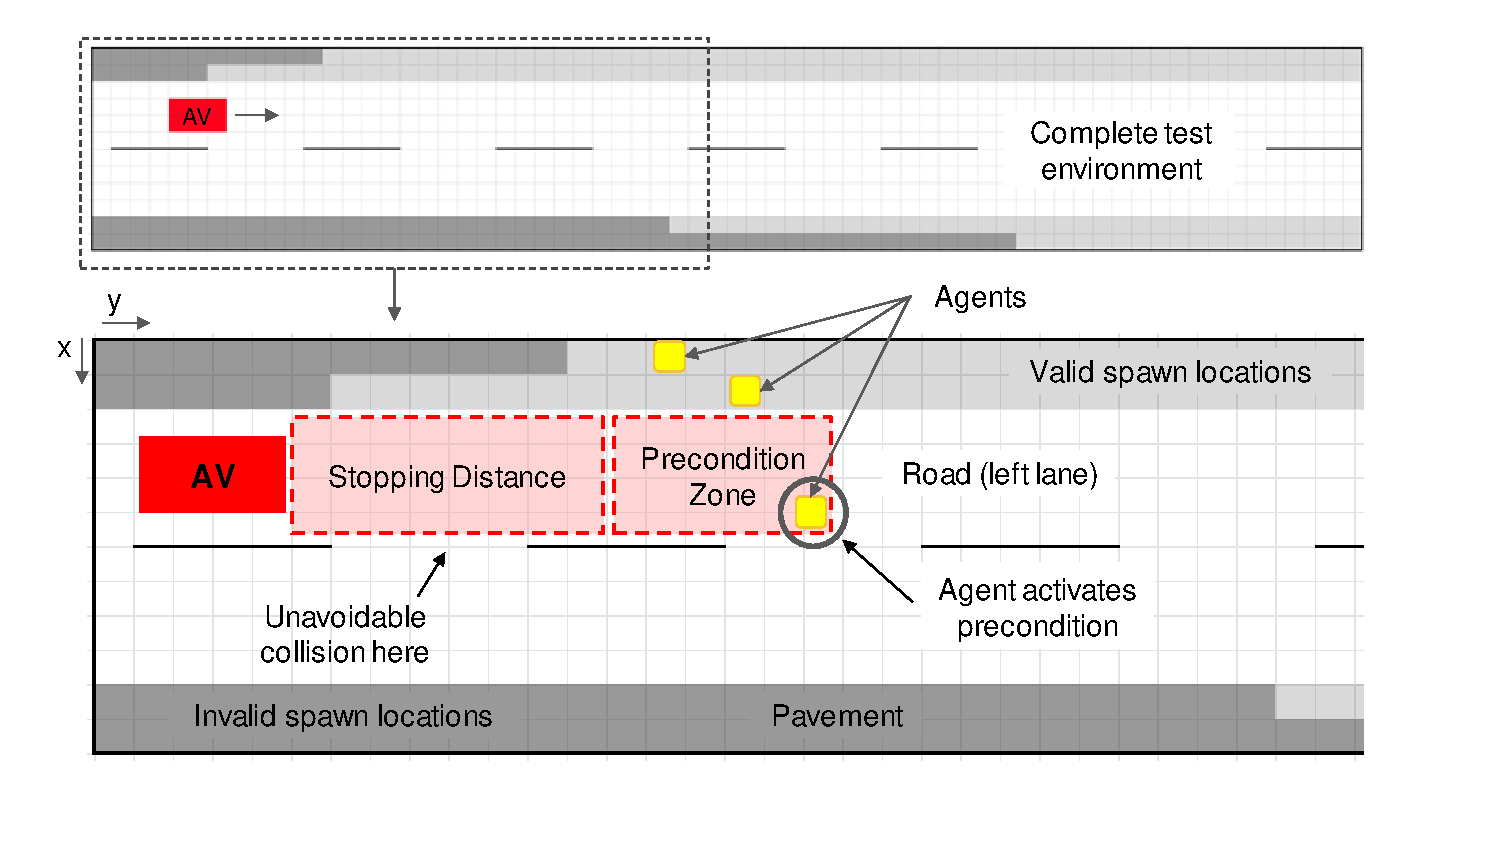
\includegraphics[width=0.48\textwidth]{RoadLayout.pdf}
	\caption{Test environment at full scale (left) and in detail (right) including valid and invalid spawn locations for the pedestrians and the position and direction of the AV.}
	\label{gridRoad}
\end{figure}



%------------------- Scoring -----------------------------
\subsection{Scoring}
Each agent behavioural method will be repeated 1000 times and the number of valid tests counted. A successful test is generated when a pedestrian intrudes into the `braking zone' of the AV that may potentially cause an intersection. %
In an attempt to impose more realistic behaviour on the agents, a scoring system is used that penalises certain actions. A living cost is imposed on the agents to promote shorter tests and a penalty is given for agents that are in the road.

The scoring system is:
\begin{itemize}
  \item A reward of 100 is given if the agent intersects the AV.
  \item A penalty of -1 for each time step.
  \item A penalty of -5 for each time step spent in the road.
\end{itemize}


%------------------- Simulation and Logging -----------------------------
\subsection{Simulation and Logging}
%Each of the agent behaviours were written into the Jason platform along with the test environment as described above. 
For each test a basic log of the agent actions, score and time to completion were recorded and then averaged for each behaviour type. A list of random start locations was created for the pedestrians and this was done for each value of $nA$ explored, i.e. 1-20. The list was then used to spawn the pedestrians for each behavioural type to ensure the initial conditions were identical. 
%
The scoring should reflect the benefits of the method against the desire to generate good tests~\cite{fewster1999software}.

% : accuracy, cost and robustness. We want tests that are accurate (valid tests, collects coverage) and sufficiently low cost (CPU hours, engineering time). If tests are robust they are adaptable to real-time events, e.g. AV slows down around bend requiring agents to recalculate intersection.

%Robustness comes from the generated tests being adaptable to non-deterministic AV behaviour, i.e. linear extrapolation of the vehicle position is not possible. The origin of the graph below identifies the lowest cost, accuracy and robustness test cases which can be attributed to random generation. By using more advanced methods we hope to improve accuracy and robustness with minimal cost.






%------------ Results Discussion ---------------
\section{Results}\label{s:results}
The results section is split into 5 parts; Accuracy is the ratio of successful tests the agents generated as a ratio of all tests, Score is a measure of how natural the agents behaved, Combined Score combines accuracy with score, and Time is how long the agents took to generate the test in both simulation ticks and wall clock time. Both Score and Time have distributions associated with them and as such confidence intervals are provided.



%--------------------------------------------------------
\subsection{Test Accuracy}
Test generation accuracy, defined as the number of tests that have activated the precondition for the assertion as a ratio of all tests, are shown for each agent type in Fig.~\ref{Accuracy}. The \textit{random} (RA) and \textit{constrained random} (CR) have lower accuracy compared to directed agents when $nA<10$. For high $nA$ the accuracies converge mostly due to a saturation of agents (explained above).
%
Fig.~\ref{Accuracy} also shows that for $nA=1$ a directed agent outperforms a random agent by more than 2:1. The \textit{election} agent generates a slightly higher accuracy than the \textit{proximity} agent but only by 2.2\%. However, for $nA=2$ and above the \textit{proximity} agent has a 10\% increase over the election agent which is because this agent has multiple attempts to trigger the precondition whereas the election agent only has one.


\begin{figure}[!t]
	\centering
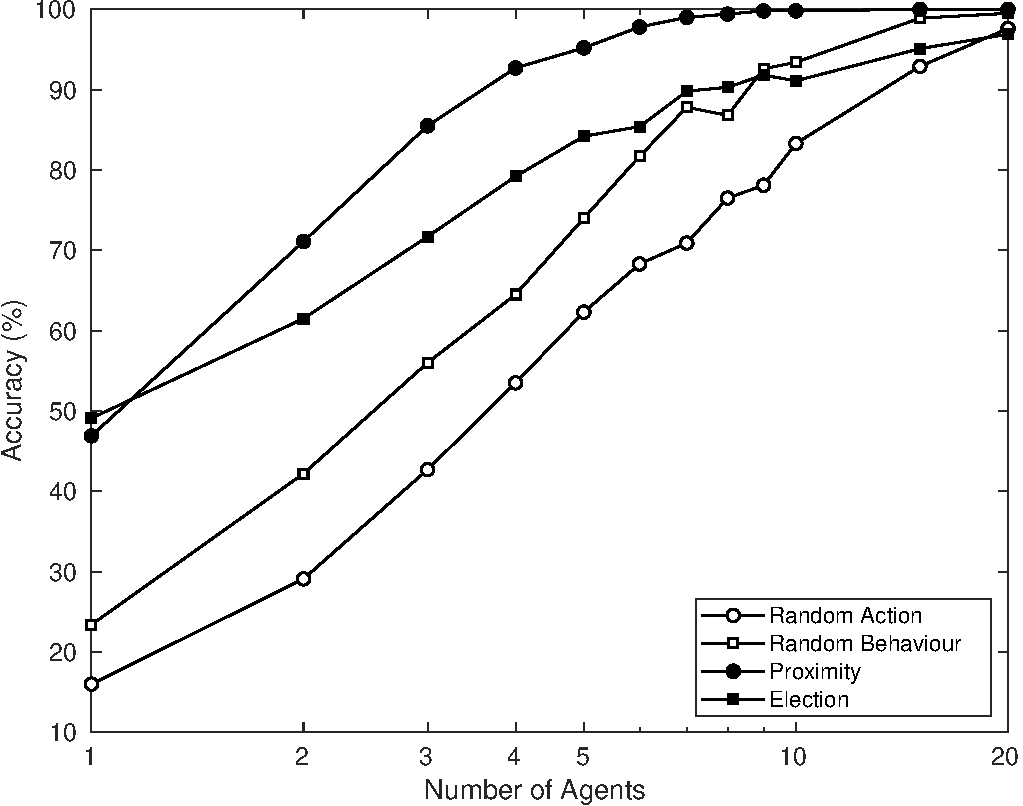
\includegraphics[width=0.48\textwidth]{Accuracy.pdf}
	\caption{Accuracy.}
	\label{Accuracy}
\end{figure}



%--------------------------------------------------------
\subsection{Test Score} \label{testscore}
For tests that activate the precondition the average agent score is compiled including 95\% confidence interval range, see Fig.~\ref{AgentScore}. The maximum theoretical score of any agent is 94 which includes 100 points for a successful test subtracting a living cost of 1 and road penalty of 5. For a single agent scores between agent types are similar as accuracy is being controlled for by including only the successful tests. As the number of agents increases the random class diverge from the directed class and the variance in the random agent score increases. 

% \todo[inline]{why no variance for nA=1 in random? this is counter intuitive, it suggests random agents that succeed score only the highest value score!} 

As $nA$ increases for the random agents, the number of agents found on the road also increases and hence average score drops rapidly, whereas the directed class are only found crossing the road when they deem fit and are on the pavement at all other times keeping the score much higher.
%
% \todo[inline]{include the theoretical max score line} Note that the directed agent class are close to the theoretical maximum score, Fig.~\ref{AgentScore}(dashed line). 
%
The high score for the $nA=1$ random class is surprising especially as the error bars are small indicating that, although the accuracy is low, tests generated are relatively efficient, i.e. the pedestrian does not spend a lot of time in the road.
%
No significant dfference between the directed class is seen in the score even with a high number of agents indicating both represent a similar level of natural behaviour, at least within the limited scope of this example.


\begin{figure}[!t]
	\centering
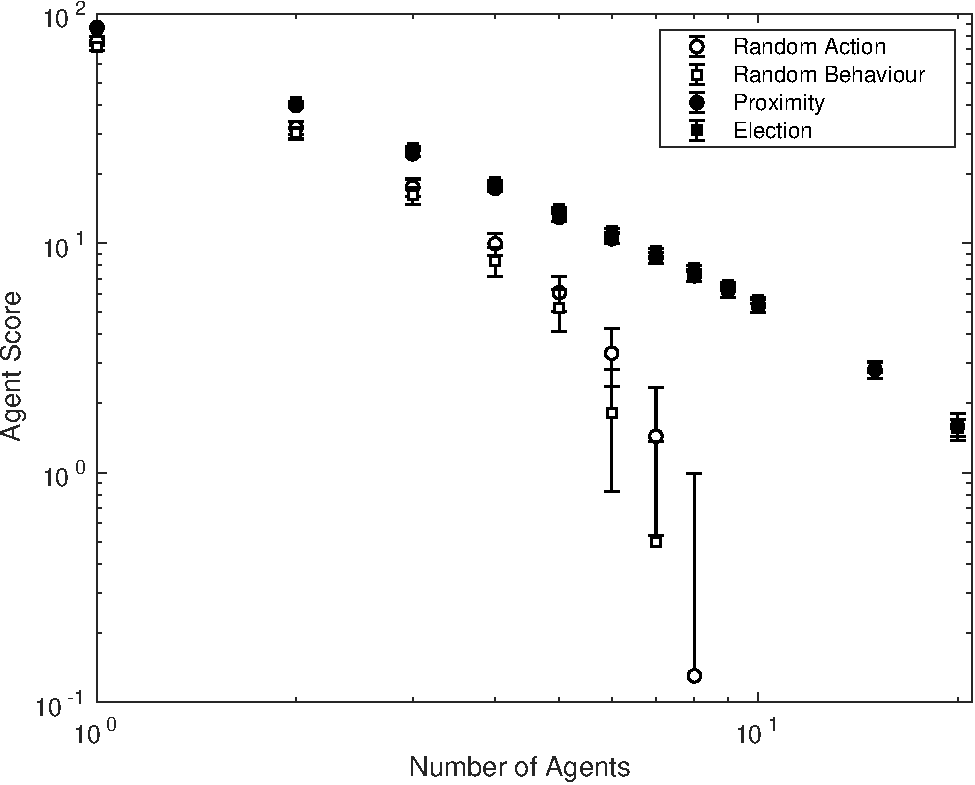
\includegraphics[width=0.48\textwidth]{AgentScore.pdf}
	\caption{The average agent score for successful tests with 95\% confidence intervals for each agent type. Random class are hollow markers and directed class are filled. The maximum theoretical score is 94 points but this is only applicable to a single agent hence the declining average with increasing agent numbers.}
	\label{AgentScore}
\end{figure}


%--------------------------------------------------------
\subsection{Combined Score}
As the score above (section \ref{testscore}) only shows tests that meet the precondition, it can be easy to interpret these results as overly optimistic so a \textit{combined score} is provided which is given by (score * accuracy / 1000). This combined measure promotes scores that are attached to high accuracies, describing agents that can generate useful tests with natural pedestrian behaviour. Time could also ave been included as a denominator here but is not as is accounted for in the living cost penalty.%
%
The normalised results, Fig~\ref{Combined}, show that the directed agents are over twice as effective within this new combined definition than random agents for $nA=1$ although this advanced drops rapidly with increasing agent numbers to reach a steady gap of around 12\%.
%
The \textit{constrained random} agent outperforms the \textit{random} for $nA<4$ beyond which there is little difference. So if random is your choice, you might as well just use completely random unless you want to use low agent numbers. %
%
The \textit{election} agent has the highest combined score for $nA=1$ but higher agent numbers are favour the \textit{proximity} agent up to $nA=4$ beyond which there is no notable difference between the directed agent types. %
%
% \todo[inline]{Describe relation to theoretical maximal?}

\begin{figure}[!t]
	\centering
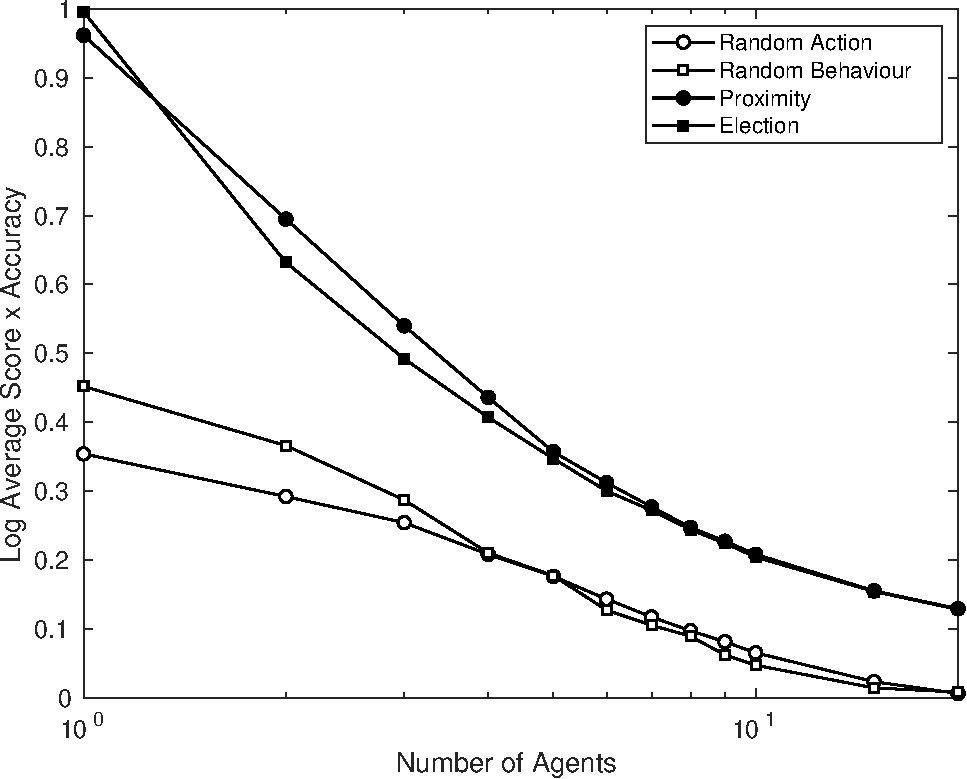
\includegraphics[width=0.48\textwidth]{Combined.pdf}
	\caption{The combined accuracy and score for each agent type.}
	\label{Combined}
\end{figure}

%\todo[inline]{y-axis is "normalised combined score" reduce height of all graphs by 30\%, change all x-axis to 1,2,3 not 10^0, add theoretical max score on this chart}


%--------------------------------------------------------
\subsection{Agent CPU Time}
% Metric of efficiency of the method, resource useage.
For each test generated that met the precondition, the CPU time taken to execute the agent action was averaged over the $k$-tests and compared across different agent types and numbers, Fig.~\ref{CPUTime}. This is essentially comparing the resources required to execute the actions of different agent types.

\begin{figure}[!t]
	\centering
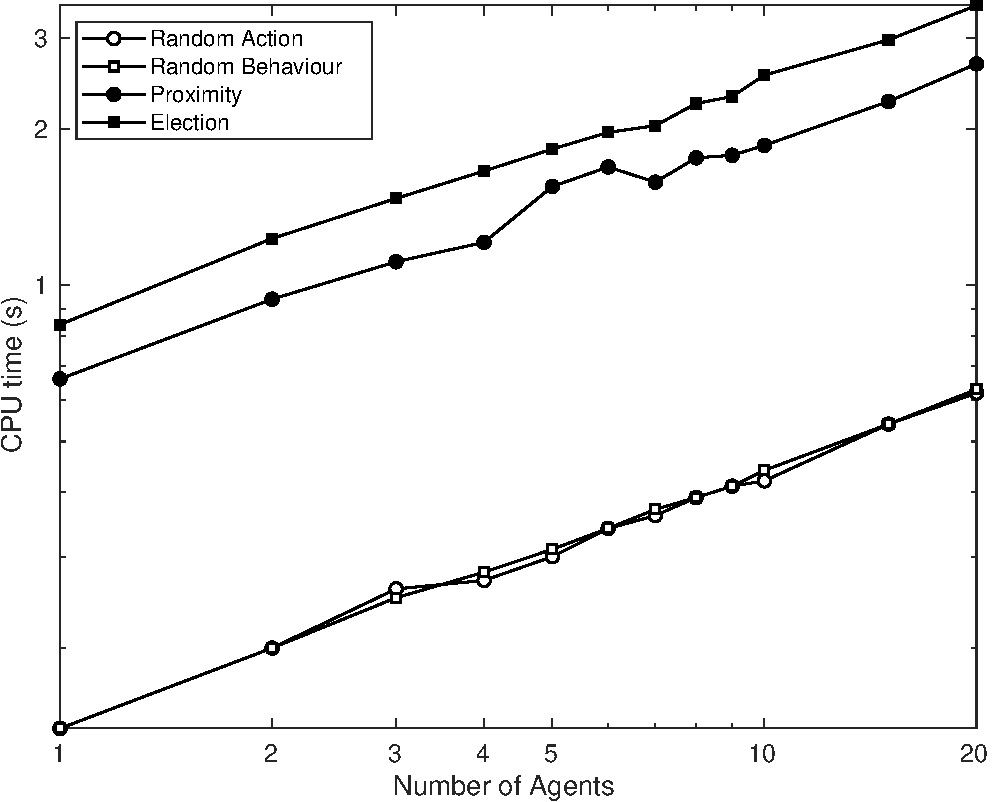
\includegraphics[width=0.48\textwidth]{TimeCPU_log.pdf}
	\caption{The CPU time taken to execute the agent actions averaged over 1000 experiments. The more complex agents have additional CPU overhead compared to random but this difference is relatively unchanged with agent numbers.}
	\label{CPUTime}
\end{figure}

% \todo[inline]{change time y-axis to sim ticks not seconds, remove valid, add wall clock time to second y-axis, add error bars to time}

%--------------------------------------------------------
%---------------- Results Table -------------------------
\begin{table*}
\centering
\caption{Test agent summary table showing description and number of lines of code ($LOC$) for each agent and sample of results: Accuracy, Combined Score ($s_c$), CPU Time ($t_{c}$) and Test Generation Time ($t_{g}$) for $nA=3$.}
\label{ResultsTable}
\begin{tabular}{|l|p{6.2cm}|c||c|c|c|c|}
\hline
\textbf{Behaviour} & \textbf{Agent Description} & $LOC$ & Accuracy (\%) & $s_c$ (points)&  $t_{c}$ (s) & $t_{g}$ (ticks) \\
\hline
Random & Randomly perform action (up, down, left, right, stop). 		&  23& 42.7 & 0.254 & 0.09 & 9.11 \\
Constrained Random & Walk along pavement, randomly cross the road 		&  82& 56.0 & 0.287 & 0.08 & 8.83 \\
Proximity & Walk along pavement, Cross road when AV in range 			&  86& 85.5 & 0.540 & 0.37 & 6.79 \\
Election & As in Proximity but elect a single agent to cross 			& 235& 71.7 & 1.470 & 0.49 & 6.59 \\
\hline 
\end{tabular}
\end{table*}

%--------------------------------------------------------
\subsection{Time to Generate Test}
% Return on investment.
For each successful test generated the reported time was averaged over $k$-tests and compared across different agent numbers, Fig.~\ref{Time}. 
%
The directed agents consistently improve over the time taken by the random class for $nA=1$ by around a single simulation tick and this trend continues as agent numbers increase. By $nA=20$ the directed agents are 1.85 simulation ticks faster than the random agents. Overall the \textit{proximity} agents find tests in the shortest number of simulation steps.

\begin{figure}[!t]
	\centering
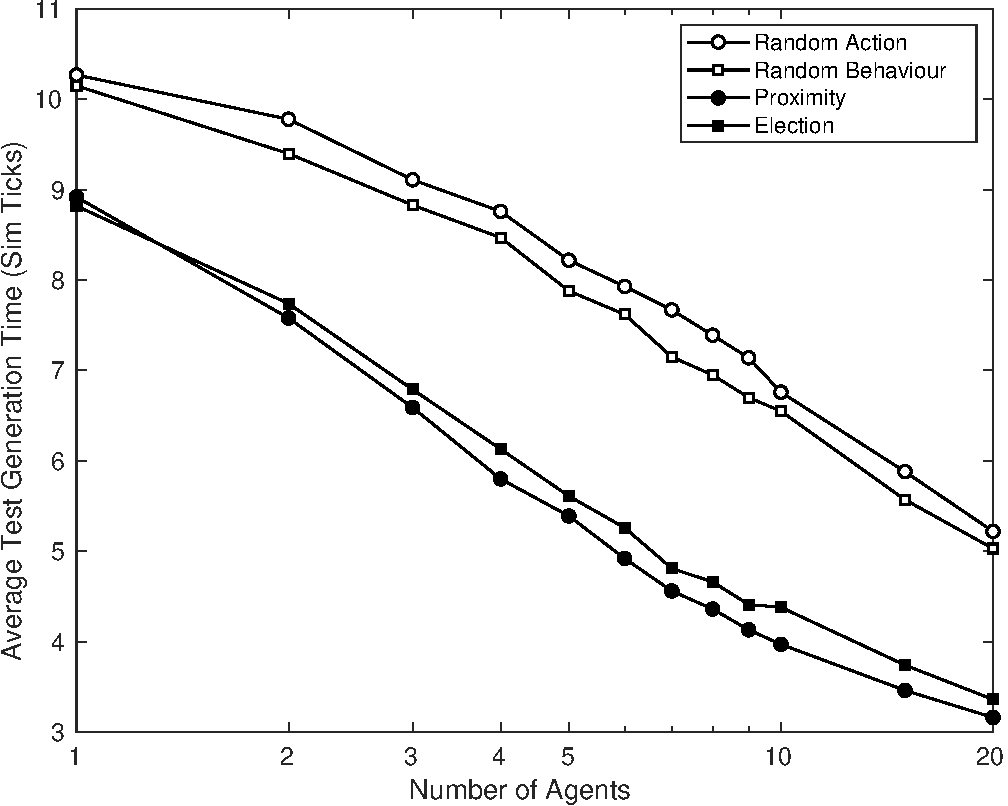
\includegraphics[width=0.48\textwidth]{Time.pdf}
	\caption{The average time taken for an agent to find a successful test, $t_{g}$.}
	\label{Time}
\end{figure}

% \todo[inline]{change time y-axis to sim ticks not seconds, remove valid, add wall clock time to second y-axis, add error bars to time}



%--------------------------------------------------------
\subsection{Results Analysis}
% \todo[inline]{discuss how the test show compliance against the `good test case' description in the intro: Accuracy is not precisely detecting defects in this case but the AV is put inot a situation where this is tested, Agent CPU is a resource metric = ecomonic, TTGT also economic but more a `return on investment' with efficiency. Agent score can be considered as the evolvable attribute as agents with a high score should do well in other environments (road layouts here) and still maintain realistic behaviour. The only attribute not covered is exemplary as in this case study only a single assertion is considered.}
% \todo[inline]{Agent density vs. accuracy - can be used to det how many agents required for map size}

The results are assessed against the criteria of a `good' test case as described in~\cite{fewster1999software}.
\begin{itemize}
	\item \textit{Effective}: How effective the method is at generating test cases that detect faults with the responder. The Accuracy metric, defined above, shows how often the agent generates a test case that satisfies the precondition of the assertion and will therefore reveal, or is likely to reveal, defects of the DUV. Fig.~\ref{Accuracy} shows that a small number of directed agents are around twice as effective as random ones and over three times as effective for a single agent.
	%
	\item \textit{Exemplary}: An exemplary test case will test multiple aspects of the DUV thereby reducing the number of tests. In this case study, only a single assertion was used so this criteria cannot be assessed although it is a key development for future work discussed in Section~\ref{s:future}.
	%
	\item \textit{Economic}: How costly the test case is to run, analyse and debug. The resource cost (CPU time) to execute the agent actions, Fig~\ref{CPUTime} is 4-5 times more expensive for the directed agents than random. An example of the actual values are given in Table~\ref{ResultsTable} $nA=3$, see heading CPU Time. This may be a significant factor in your decision to use an intelligent agent for test generation unless you have abundant CPU resources to hand. %
	%
	However, the test generation time, Fig~\ref{Time}, indicates that on average the directed agents find test cases that activate the precondition faster than random in terms of simulation ticks. Therefore, although more resource is allocated to the directed agents they find tests faster overall due to better efficiency, i.e. better return on investment (ROI).
	%
	\item \textit{Evolvable}: The maintenance required to adapt the test case to new software changes or \textit{scenes} in our case. In the case study each test generated is of a different scene as the agent position is randomly generated each time. Therefore the directed agents show adaptability to new scenes and this attribute is accounted for within the accuracy. This case study could be easily shown to succeed with different road layouts, vehicle speeds, see Section~\ref{s:future}.
\end{itemize}

% \todo[inline]{Do we need to add a new category to this list Eathly, Existent (def.=having reality), Embodied?-  level of natural or expected behaviour? Test cases generated may be both valid and interesting but not realistic - how do we control for this? do we need to? or does it not matter?}

Further to this list of attributes, some generated tests may be \textit{valid} and \textit{interesting} but may not be \textit{realistic} i.e. a \textit{valid} test could technically happen but might never occur in reality. For example, a test that generated a vehicle driving in a river or parked on a building are invalid however a car driving the wrong way down a motorway/highway is valid but unrealistic. %
% \todo[inline]{Or is this just an example of an extreme edge case? Comments welome here as i'm not convinced of my own arguemnt! I suppose if you can you generate the same test in multiple ways then you should choose one that is more realistic.} %
Therefore the category \textit{Existent} should be added:
\begin{itemize}
	% \item \textit{Existent}: The level of reality of the test case beyond simply being valid. Agents in this case study are penalised for walking in the road, see Fig.~\ref{AgentScore}.
	% \item or...
	\item \textit{Existent}: Test cases should promote realistic scenarios or if competing valid cases exist then deference should be given to the more realistic one. Agents in this case study are penalised for walking in the road, see Fig.~\ref{AgentScore}.
\end{itemize}


The results show that by nearly all the metrics and parameter combinations discussed above, (accuracy, natural behaviour score, test generation time) the directed agents outperform the random agents. This shows that even a small amount of intelligence can be a distinct advantage over random techniques. 
%

% This need to be added to the economic alanysis above
But what was the cost of developing these agent behaviours and is there a limited pay-off to gain significantly superior intelligence for really complex agent behaviour? %
%
Comparing the lines of code for each agent can help to weigh the investment in agent complexity, see lines of code ($LOC$) in Table~\ref{ResultsTable}. This shows that for a small investment the \textit{random} agent with 23 lines of code can be improved significantly with (86 lines) to improve it's combined score and test generation time ($t_{g}$). To improve the combined score further with the \textit{election} agent took 10x the \textit{random} code with lower overall accuracy but better combined score suggesting this was not worth the investment.

% This also raises the question of how comlex the agents sould be? 
This analysis above would suggest that the level of agent complexity should be considered carefully as a simpler level of intelligence could be more beneficial than very complex one which may also required additional investment in debugging.





%----------------- Conclusion ---------------------------
\section{Conclusion and Future Work}\label{s:conclusion}
The MAS programming paradigm offers rational agency and strategic planning to software agents that have been exploited in this research for test generation. 
%
On a small example we show that, by encoding a variety of different behaviours respondent to the agent's perceptions of the test environment, the agent-based approach generates twice as many effective tests than a pseudo-random approach. Furthermore, agents can be encoded to behave more realistically without compromising their effectiveness. %
% I think this shouldbe changed  to state:
% Our results suggest that generating tests using testing agents allows engineers to reach edge cases and rare events more easily.
Our results suggest that generating tests using testing agents is a promising avenue of research and has been shown to significantly improves upon random whilst simultaneously providing more realistic driving scenarios.



% \subsection{Future Work} 
%
% In this case study there is only a single assertion considered. But 
Future work will consider how agents behave when multiple assertions %or \textit{desires} 
exist in a variety of different scenes. %will be key to the success of this method. 
% This could be achieved with a number of methods such as MDP and ANN. 
% Furthermore, testing the agents in a variety of different scenes (e.g. different road network) would further validate the directed agent approach.
As discussed in~\cite{Eder2007} agents could have their goal selection modified based on coverage feedback %would be an important step in this direction. This also 
which fits in with the feedback reward of many such architectures, e.g. MDP~\cite{littman1994markov} and back-propagation for ANN~\cite{foerster2016learning}. %
%
Abstracting agent perceptions to a feature based representation would ensure the agent state space can scale to large physical maps and is adaptable to new features as more assertions are added. %This approach also fits in with most ML techniques.
Including personality to agents is also another avenue that could provide insightful as a tuning parameter~\cite{Zoumpoulaki2010} to explore edge cases. %Conventionally agressive (or egoist) behaviour may seem the most interesting as edge cases and therefore require oversampmling. But there could also be merit in exploring more risk-advers behaviours or simply in understanding what normative driving conditions are as a baseline for CAV cyber security. 
% There is also the possibility to have have combination of random and directed agents to ensure the initial 80\% of coverage is satisfied quickly then add more intelligent agents for hole coverage.

% \todo{without millions of miles of testing?}


%----------------- Acknowledgment ---------------------------
\section*{Acknowledgement}
This research has in part been funded by the ROBOPILOT and CAPRI projects. Both
projects are part-funded by the Centre for Connected and Autonomous
Vehicles (CCAV), delivered in partnership with Innovate UK under grant numbers
103703 (CAPRI) and 103288 (ROBOPILOT), respectively.

% We gratefully acknowledge the support of NVIDIA Corporation with the donation of a Titan Xp GPU used for this research.

%----------------- Bibliography ---------------------------
\balance
\section*{References}
\printbibliography[heading=none]
\end{document}



% ensure readeris aware it is a fake AV not a real one
% map has non-traversible boundaries, no agents lost or created, define situation/scenario in terms of each test
% test can be regenerated exactly due to seed control
